% Template:     Informe LaTeX
% Documento:    Archivo de ejemplo
% Versión:      7.0.0 (23/06/2020)
% Codificación: UTF-8
%
% Autor: Pablo Pizarro R.
%        Facultad de Ciencias Físicas y Matemáticas
%        Universidad de Chile
%        pablo@ppizarror.com
%
% Manual template: [https://latex.ppizarror.com/informe]
% Licencia MIT:    [https://opensource.org/licenses/MIT]

% ------------------------------------------------------------------------------
% NUEVA SECCIÓN
% ------------------------------------------------------------------------------
% Las secciones se inician con \section, si se quiere una sección sin número se
% pueden usar las funciones \sectionanum (sección sin número) o la función
% \sectionanumnoi para crear el mismo título sin numerar y sin aparecer en el índice

\newcommand{\explorelite}{\textit{explore\_lite}}
\newcommand{\movebase}{\textit{move\_base}}

\section{Pregunta 1}

\subsection{Parte a.-}

Se construyó el bloque de transformada $abc$ a $dq$ de manera análoga para las señales de voltaje y corriente. Externamente el bloque se ve así:

\begin{figure}
    \centering
    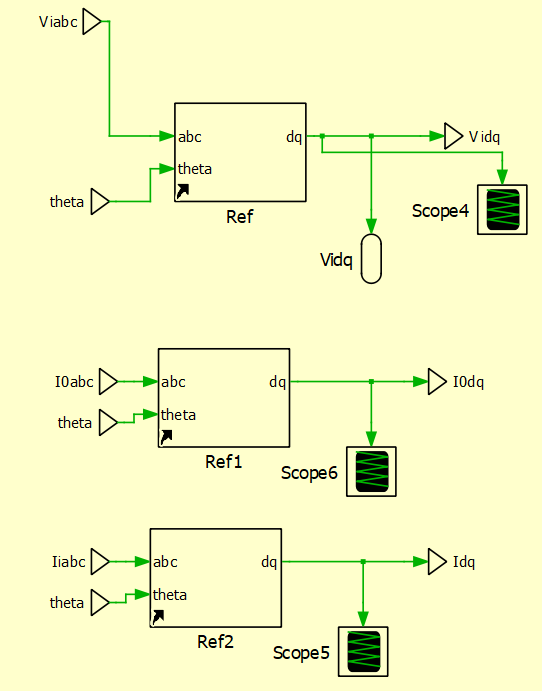
\includegraphics[width=0.5\linewidth]{Tarea 1/report/imagenes/p1a/transformadaporfuera.png}
    \caption{Perspectiva externa del bloque de la transformada $abc$-$dq$.}
    \label{transformadaporfuera}
\end{figure}

Dentro del bloque, se puede visualizar lo siguiente:

\begin{figure}
    \centering
    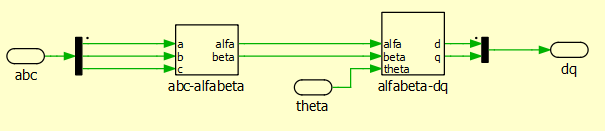
\includegraphics[width=0.5\linewidth]{Tarea 1/report/imagenes/p1a/transformadapordentro.png}
    \caption{Perspectiva interna del bloque de la transformada $abc$-$dq$.}
    \label{transformadapordentro}
\end{figure}

A partir de la Figura \ref{transformadapordentro}, se pueden ver los bloques de transformada $abc$-$\alpha\beta$ y $\alpha\beta$-$dq$. Estos bloques se armaron de la siguiente forma:

\begin{itemize}
    \item $abc$-$\alpha\beta$:

    \begin{figure}
       \centering
       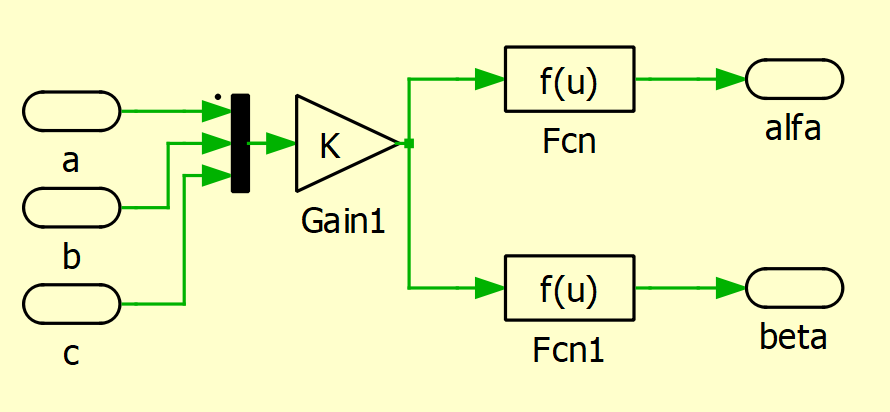
\includegraphics[width=0.5\linewidth]{Tarea 1/report/imagenes/p1a/abc-alphabetha.png}
       \caption{Bloque de transformada $abc$-$\alpha\beta$.}
       \label{abc-alphabetha}
    \end{figure}

    \begin{figure}
       \centering
       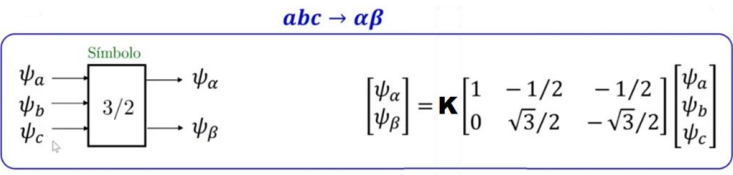
\includegraphics[width=0.5\linewidth]{Tarea 1/report/imagenes/p1a/formulaabc-alphabetha.png}
       \caption{Transformación matemática $abc$-$\alpha\beta$.}
       \label{formulaabc-alphabetha}
    \end{figure}

    De acuerdo a lo visto en clases, a las señales $abc$ se les aplicó la transformación que se visualiza en la Figura \ref{formulaabc-alphabetha} para dar origen al dominio $\alpha\beta$ como se puede ver en la Figura \ref{abc-alphabetha}, donde el valor de $K$ fue inicializado en $\frac{2}{3}$, el bloque ``Fcn'' equivale a las operaciones matemáticas que dan origen a la primera fila de la matriz $\alpha\beta$ y el bloque ``Fcn1''  equivale a las operaciones matemáticas que dan origen a la segunda fila de la matriz $\alpha\beta$.

    \item $\alpha\beta$-$dq$:

    \begin{figure}
       \centering
       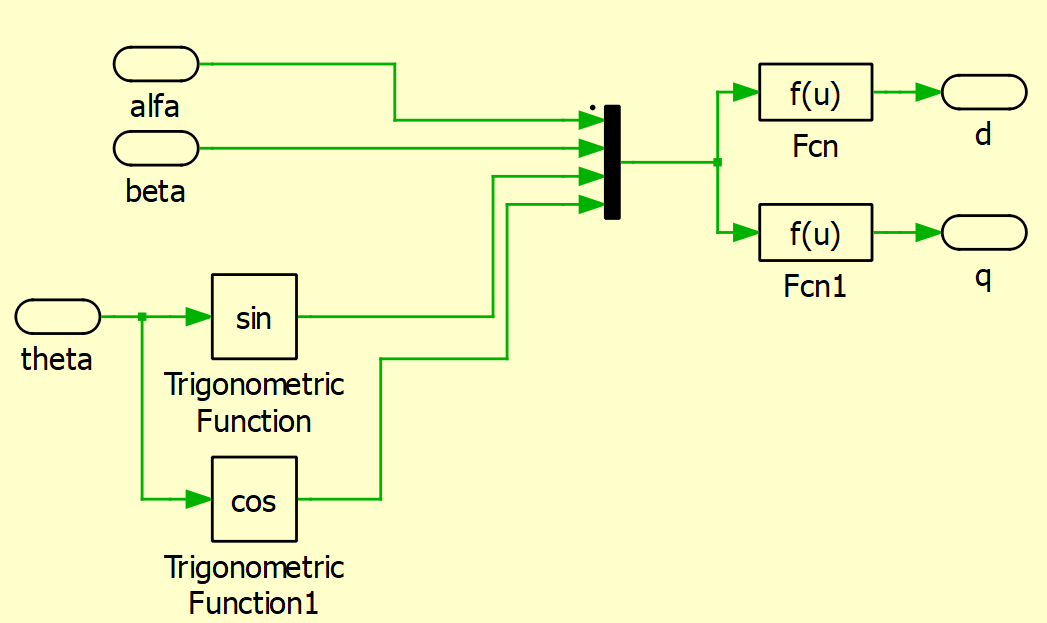
\includegraphics[width=0.5\linewidth]{Tarea 1/report/imagenes/p1a/alphabetha-dq.png}
       \caption{Bloque de transformada $\alpha\beta$-$dq$.}
       \label{alphabetha-dq}
    \end{figure}

    \begin{figure}
       \centering
       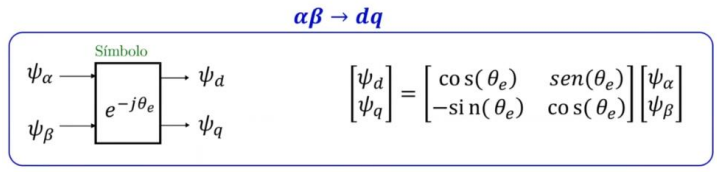
\includegraphics[width=0.5\linewidth]{Tarea 1/report/imagenes/p1a/formulaalphabetha-dq.png}
       \caption{Transformación matemática $\alpha\beta$-$dq$.}
       \label{formulaalphabetha-dq}
    \end{figure}

    De acuerdo a lo visto en clases, a las señales $\alpha\beta$ se les aplicó la transformación que se visualiza en la Figura \ref{formulaalphabetha-dq} para dar origen al dominio $dq$ como se puede ver en la Figura \ref{alphabetha-dq}, donde el bloque ``Fcn'' equivale a las operaciones matemáticas que dan origen a la primera fila de la matriz $dq$ y el bloque ``Fcn1''  equivale a las operaciones matemáticas que dan origen a la segunda fila de la matriz $dq$.
\end{itemize}

Cabe destacar que la idea de realizar la transformación del dominio $abc$ al dominio $dq$ es meramente por simplificación dado que se permite tratar los valores de voltaje y corriente como variables de corriente continua (DC).

\subsection{Parte b.-}

Utilizando las coordenadas $dq$, se creó el siguiente bloque capaz de hacer el cálculo de potencia activa y reactiva:

\begin{figure}
    \centering
    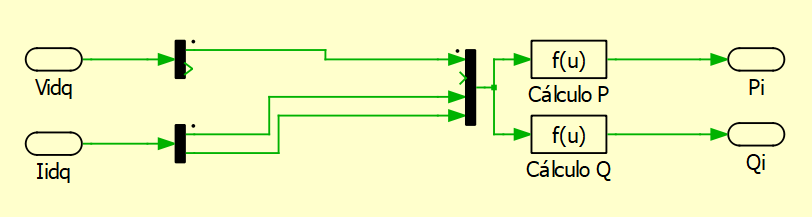
\includegraphics[width=0.5\linewidth]{Tarea 1/report/imagenes/p1b/bloquepq.png}
    \caption{Bloque que calcula la potencia activa y reactiva en base a las variables de voltaje corriente en el dominio $dq$.}
    \label{bloquepq}
\end{figure}

Como se puede visualizar en la Figura \ref{bloquepq}, el multiplexor tiene 4 entradas pero la segunda no recibe nada, esto ocurre debido a que el al alinear el sistema de coordenadas $dq$ con la dirección de la tensión (en particular, con el eje $d$), se logra que el voltaje en el eje $q$ sea 0, lo cual permite una separación clara entre la potencia activa y la reactiva, simplificando el control de la potencia en sistemas de conversión de energía. En otras palabras, se requiere que el voltaje en el eje $q$ sea 0. Luego, se siguen las siguientes fórmulas para el cálculo de P y Q:

\begin{equation}
    P = kv_{d}i_{d}
\end{equation}

\begin{equation}
    Q = -kv_{d}i_{q}
\end{equation}

Estas fórmulas se encuentran contenidas en los bloques ``Cálculo P'' y ``Cálculo Q'' respectivamente.

\subsection{Parte c.-}

Externamente, el bloque dentro del diagrama se puede visualizar de la siguiente forma:

\begin{figure}
   \centering
   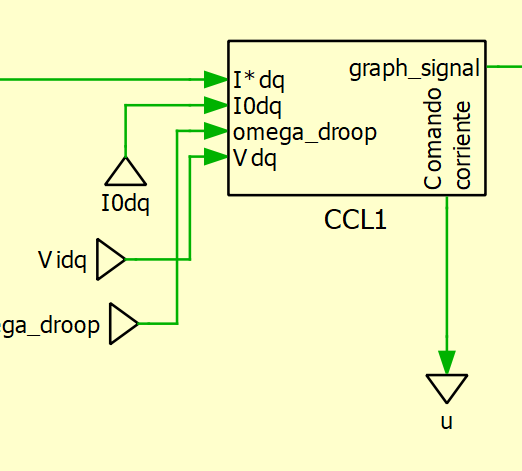
\includegraphics[width=0.5\linewidth]{Tarea 1/report/imagenes/p1c/ccl bloque externo.png}
   \caption{Perspectiva externa del bloque de control del lazo de corriente.}
   \label{ccl externo}
\end{figure}

Internamente, se utilizó un control con términos cruzados visto en cátedra, tal como se puede ver en la siguiente figura:

\begin{figure}
   \centering
   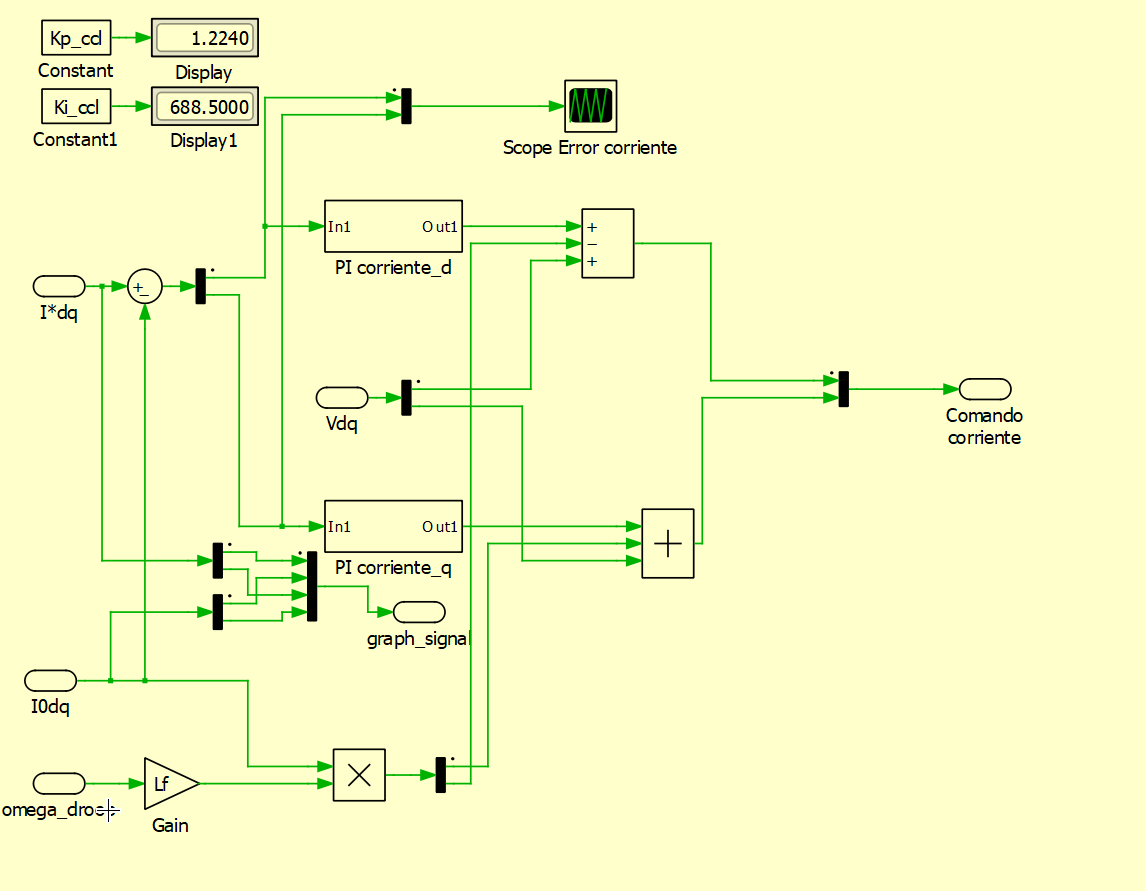
\includegraphics[width=0.5\linewidth]{Tarea 1/report/imagenes/p1c/ccl bloque interno.png}
   \caption{Perspectiva interna del bloque de control del lazo de corriente.}
   \label{ccl interno}
\end{figure}

De acuerdo a lo visto en clases, a cada lazo de control primario se le dio como entrada un escalón con el fin de poder sintonizar los valores de las constantes proporcionales e integrales de los controladores PI, en función del valor de \textit{overshoot} y tiempo de estabilización observado. La respuesta obtenida se pueden observar en la figura \ref{step_response_ccl}. Las fórmulas utilizadas para definir estos valores fueron:

\begin{equation}
    k_p^i = 2L\zeta w_{n}
\end{equation}

\begin{equation}
    k_i^i = Lw_{n}^2
\end{equation}

considerando $\omega_n$ como la frecuencia natural del controlador y $\zeta$ como coeficiente de amortiguamiento. Utilizando estas fórmulas, se determinó que los valores de $k_p^i$ y $k_i^i$ son 1.224 y 688.5 respectivamente, utilizando un $\zeta$ de 0.8 y un $w_{n}$ de 900Hz. Estos coeficientes fueron usados para los controladores tanto de la corriente en d como en q.

\begin{figure}
   \centering
   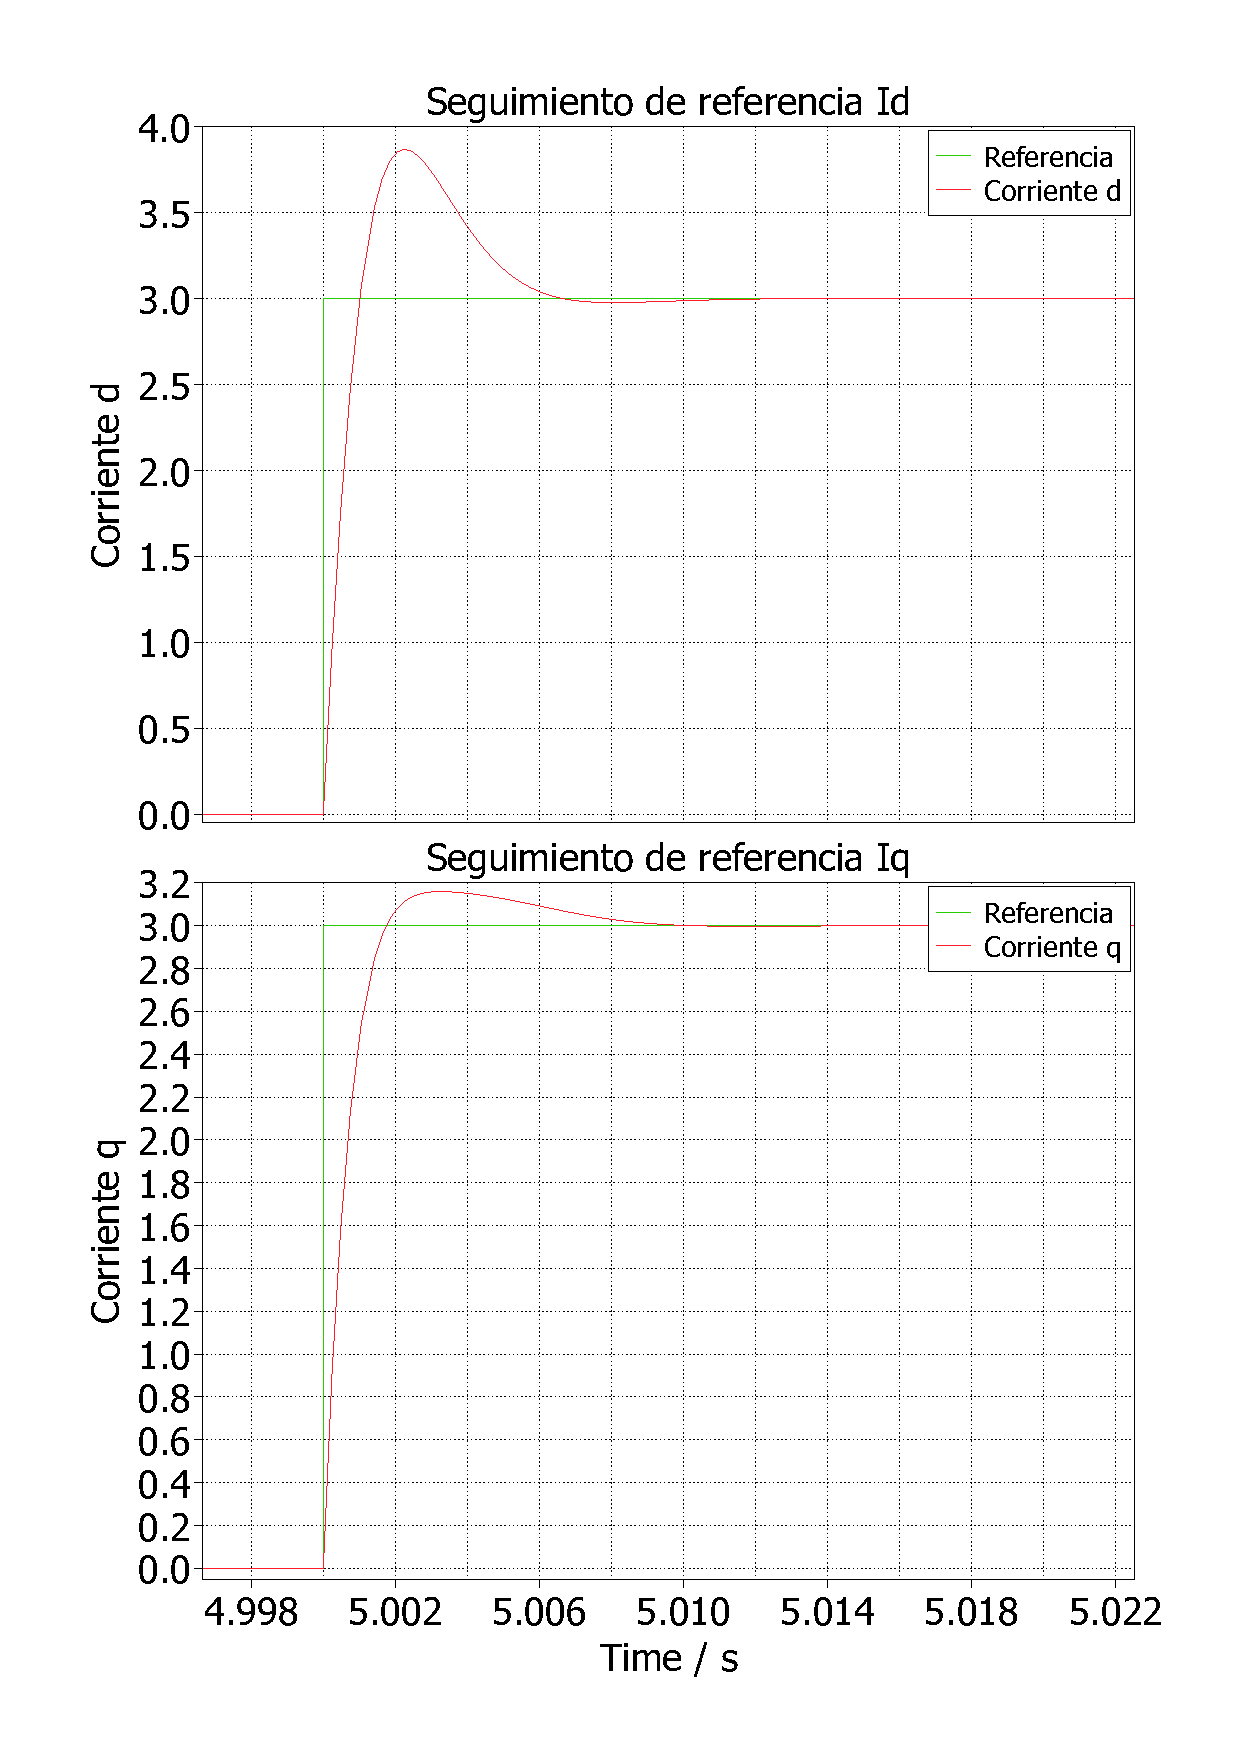
\includegraphics[width=0.5\linewidth]{Tarea 1/report/imagenes/p1c/respuesta_escalon_ccl.pdf}
   \caption{Respuesta al escalón de lazo de control de corriente.}
   \label{step_response_ccl}
\end{figure}

\subsection{Parte d.-}

Externamente, el bloque dentro del diagrama se puede visualizar de la siguiente forma:

\begin{figure}
   \centering
   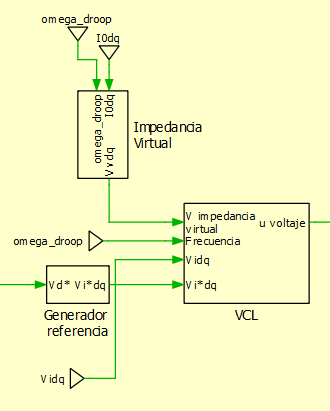
\includegraphics[width=0.5\linewidth]{Tarea 1/report/imagenes/p1d/vcl bloque externo.png}
   \caption{Perspectiva externa del bloque de control del lazo de voltaje.}
   \label{vcl externo}
\end{figure}

Internamente, se utilizó un control con términos cruzados visto en cátedra, tal como se puede ver en la siguiente figura:

\begin{figure}
   \centering
   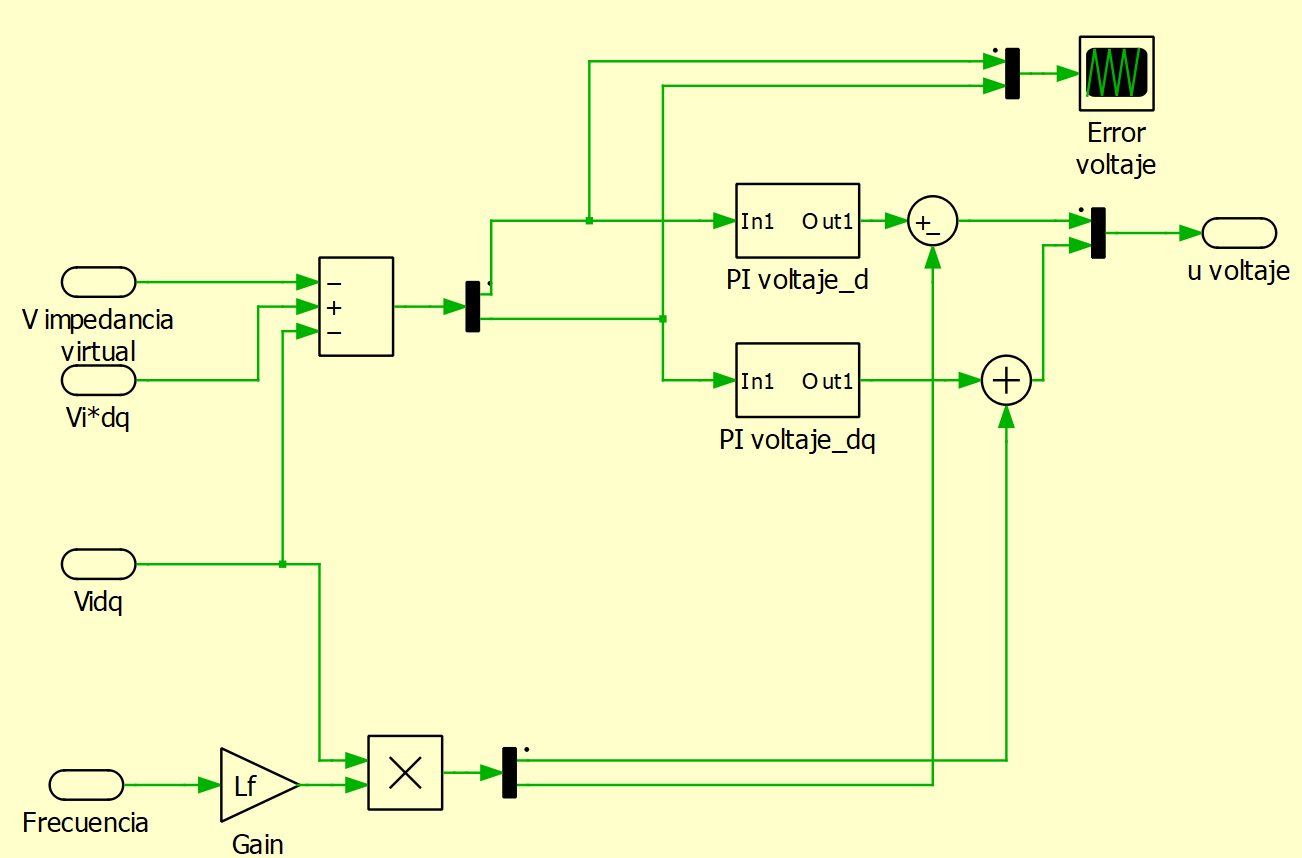
\includegraphics[width=0.5\linewidth]{Tarea 1/report/imagenes/p1d/vcl bloque interno.png}
   \caption{Perspectiva interna del bloque de control del lazo de voltaje.}
   \label{vcl interno}
\end{figure}

De acuerdo a lo visto en clases, al modelo físico se le dio de entrada un escalón con el fin de observar su comportamiento, de esta manera fue posible estipular los valores de las constantes proporcionales e integrales de los controladores PI para cada entrada de voltaje en el dominio $dq$, las fórmulas utilizadas para definir estos valores fueron:

\begin{equation}
    k_p^v = 2C\zeta w_{n}
\end{equation}

\begin{equation}
    k_i^v = Cw_{n}^2
\end{equation}

Utilizando estas fórmulas, se determinó que los valores de $k_p^v$ y $k_i^v$ son 0.0088 y 0.343 respectivamente, utilizando un $\zeta$ de 0.9 y un $w_{n}$ de 70Hz. Estos coeficientes fueron usados para los controladores de voltaje tanto en d como en q. 

La frecuencia natural escogida se eligió de tal forma que fuera como mínimo 10 veces más pequeña que aquella del lazo de corriente, con el objetivo de desacoplar los lazos de control. Luego, tanto esta como el coeficiente de amortiguamiento fueron seleccionados de tal forma de reducir lo más posible el error estacionario y reducir el valor del \textit{overshoot} frente a un escalón. La simulación obtenida se puede observar en la figura \ref{step_response_vcl}.


\begin{figure}
   \centering
   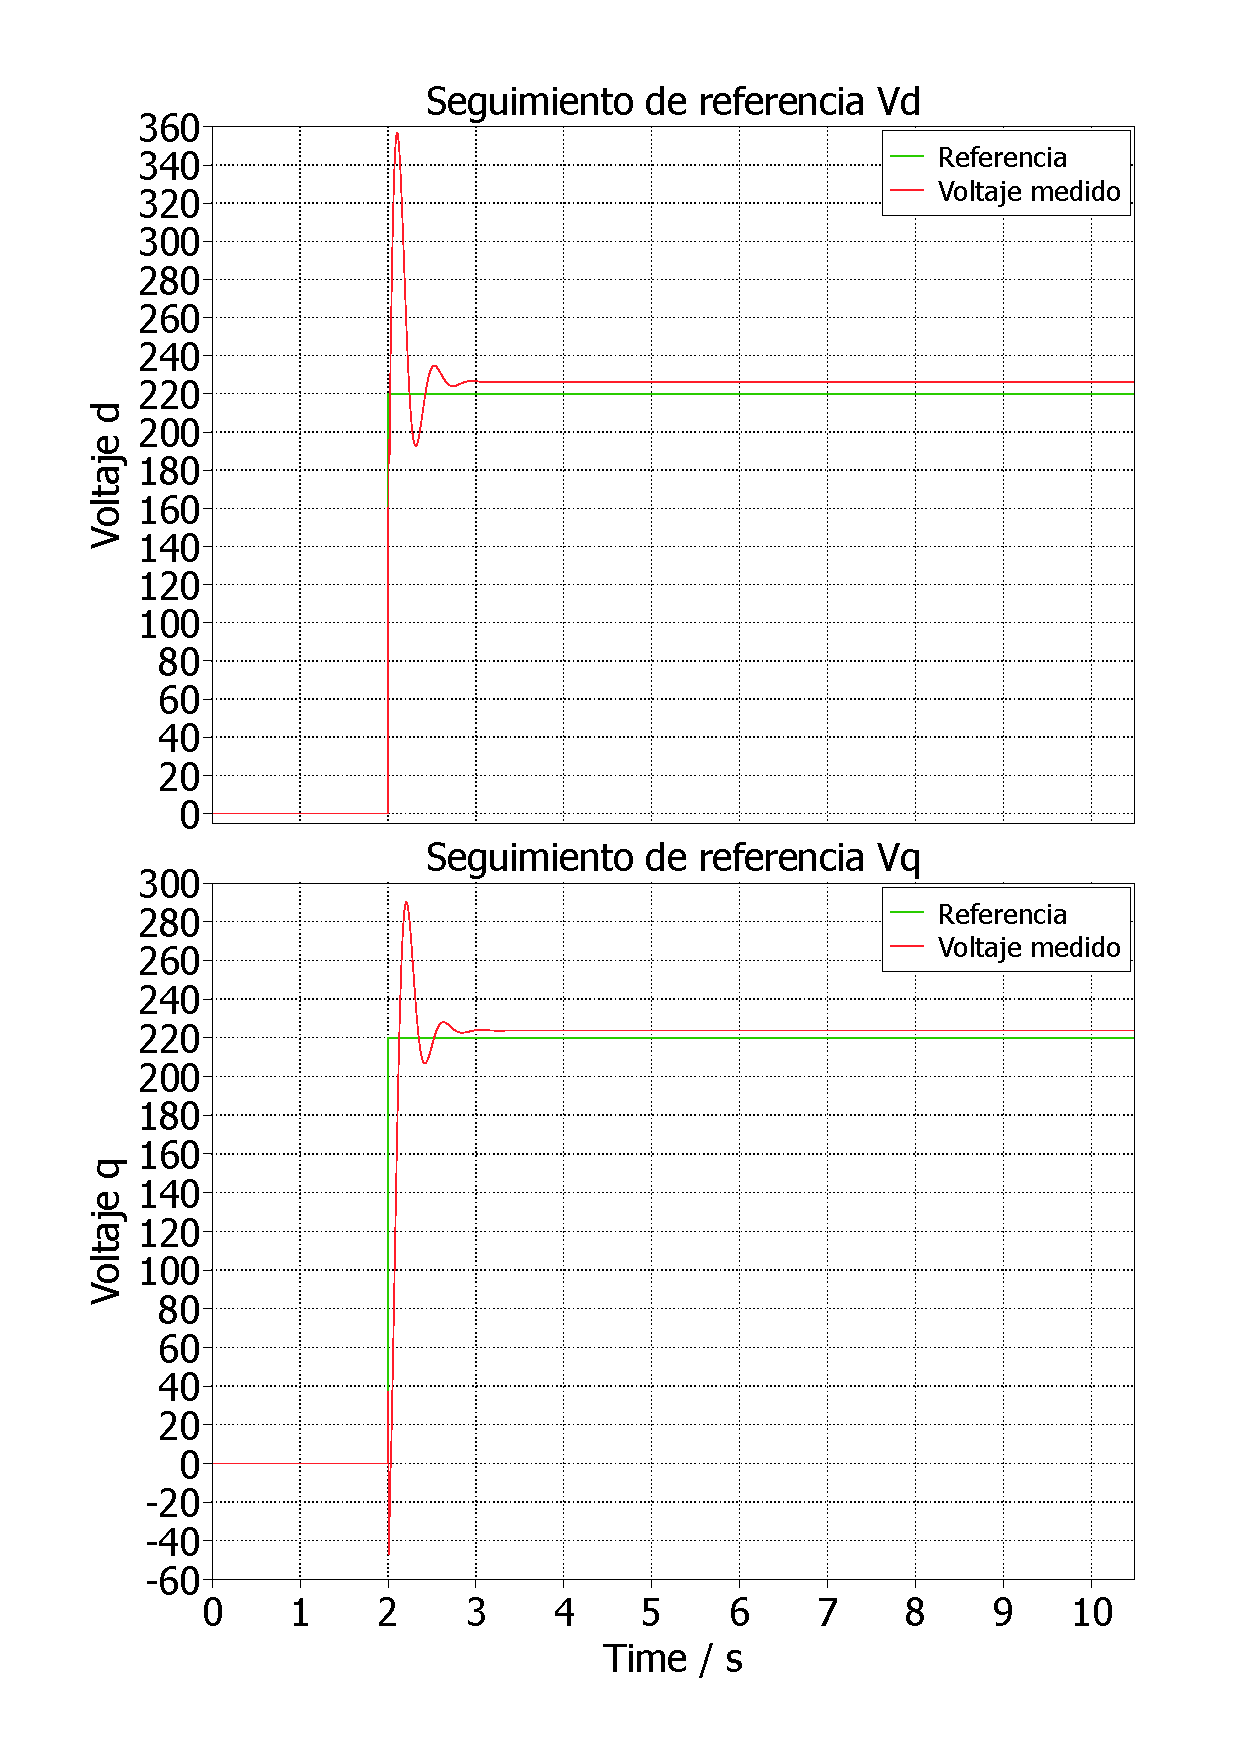
\includegraphics[width=0.5\linewidth]{Tarea 1/report/imagenes/p1c/respuesta_escalon_vcl.pdf}
   \caption{Respuesta al escalón de lazo de control de tensión.}
   \label{step_response_vcl}
\end{figure}

\subsection{Parte e.-}
Considerando los rangos de coeficiente de amortiguamiento y frecuencia recomendados para el lazo de control de corriente, se obtuvo la respuesta de la figura \ref{step_response_ccl}. Esta figura corresponde a la de los valores que causaron el menor \textit{overshoot} observado, con un valor de aproximadamente 23\% para la corriente d, 6\% y un tiempo de estabilización de 0.01 segundos para ambos.  

\section{Pregunta 2}

\subsection{Parte a.-}

De acuerdo a lo visto en clases, para calcular la pendiente droop para cada potencia se debe seguir las siguientes fórmulas:

\begin{equation}
    M_p = \frac{\Delta w}{P_{máx}}
\end{equation}

\begin{equation}
    M_q = \frac{\Delta w}{Q_{máx}}
\end{equation}

En nuestra implementación se optó por crear un subsistema con parámetros regulables a través del diálogo de la figura \ref{dialogo_dg}, por lo que se usa internamente las siguientes fórmulas:

\begin{equation*}    
M_p = -\omega_0\frac{(\Delta_\omega)}{100\cdot P_{max}};
\end{equation*}

\begin{equation*}
M_q = -V_0\frac{(\Delta_V)}{100\cdot Q_{max}};
    
\end{equation*}

donde $\Delta_V$ y $\Delta_\omega$ son valores dentro de los rangos estipulados en el enunciado de la tarea: $[0.1 - 30]$ para la frecuencia; $[0.1 - 10]$ para la tensión. Se consideró inicialmente una variación de frecuencia de 5\% y de voltaje de 2\%, obteniéndose las pendientes droop $M_p = -1.6\cdot 10^{-4}$ y $ Mq = -7.33 \cdot 10^{-4}$.\\

\begin{figure}
   \centering
   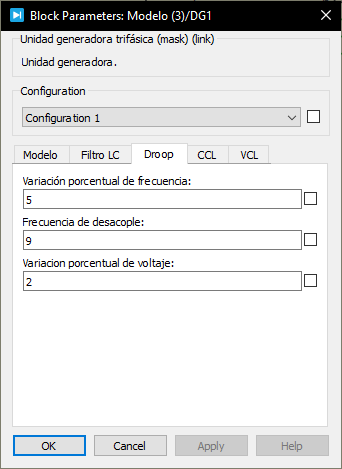
\includegraphics[width=0.5\linewidth]{Tarea 1/report/imagenes/p2a/dialogo_dg.png}
   \caption{Diálogo de parametrización de variables \textit{droop}.}
   \label{dialogo_dg}
\end{figure}

Al realizar una simulación teniendo las 3 máquinas generadoras con la misma pendiente droop de potencia activa y reactiva, se obtuvieron los siguientes resultados:

\begin{figure}
   \centering
   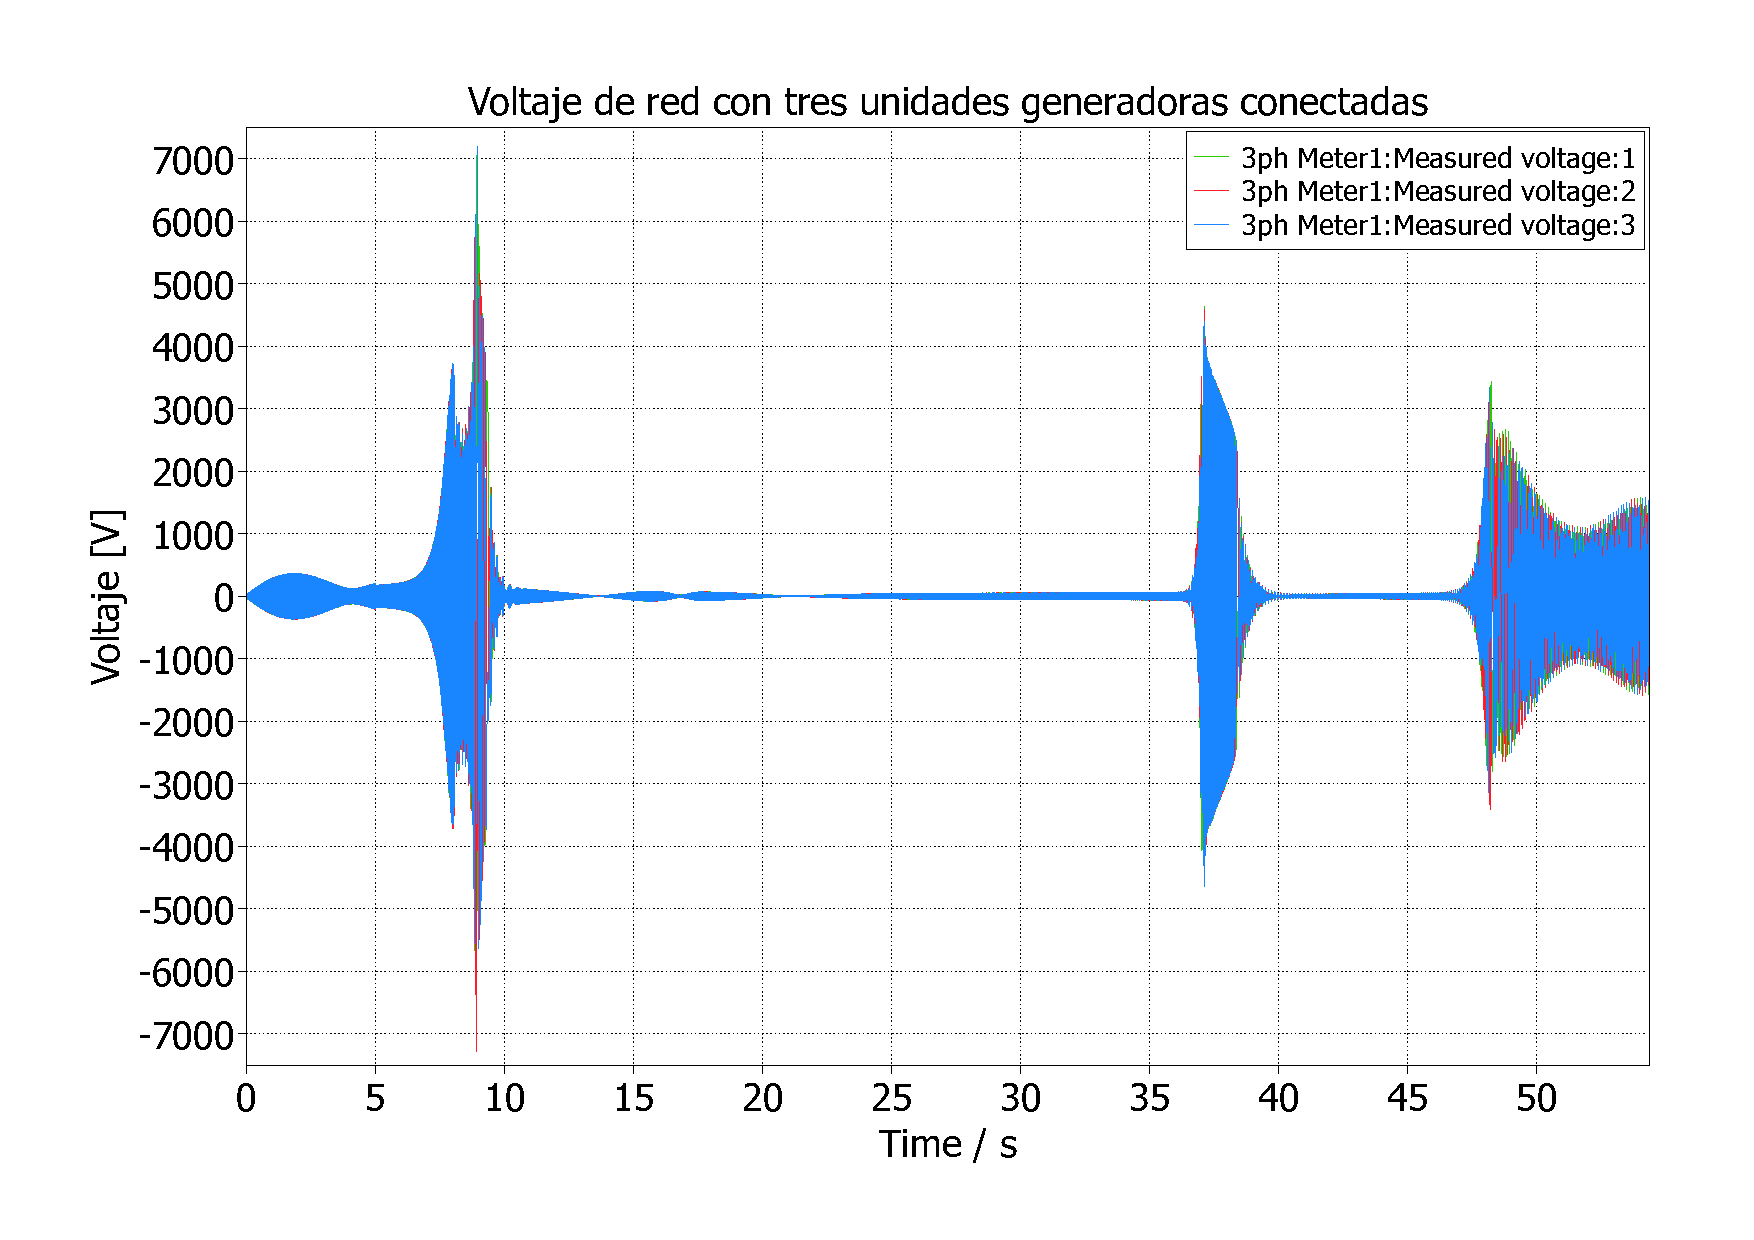
\includegraphics[width=0.5\linewidth]{Tarea 1/report/imagenes/p3a/resonancia_generadores.pdf}
   \caption{Diálogo de parametrización de variables \textit{droop}.}
   \label{resonancia_generadores}
\end{figure}

Se observa en la figura \ref{resonancia_generadores} que los generadores no logran mantener el voltaje dentro de un rango razonable en torno al voltaje nominal, que es lo que se hubiera esperado. Debido a esto, resulta imposible estudiar el efecto de la conexión y desconexión de cargas. Sin embargo, se puede estudiar el efecto del cambio de las pendientes \textit{droop} de una sola unidad generadora. A partir de esto se obtienen las figuras \ref{droop_1}, \ref{droop_́2} y \ref{droop_3}.


\begin{figure}
   \centering
   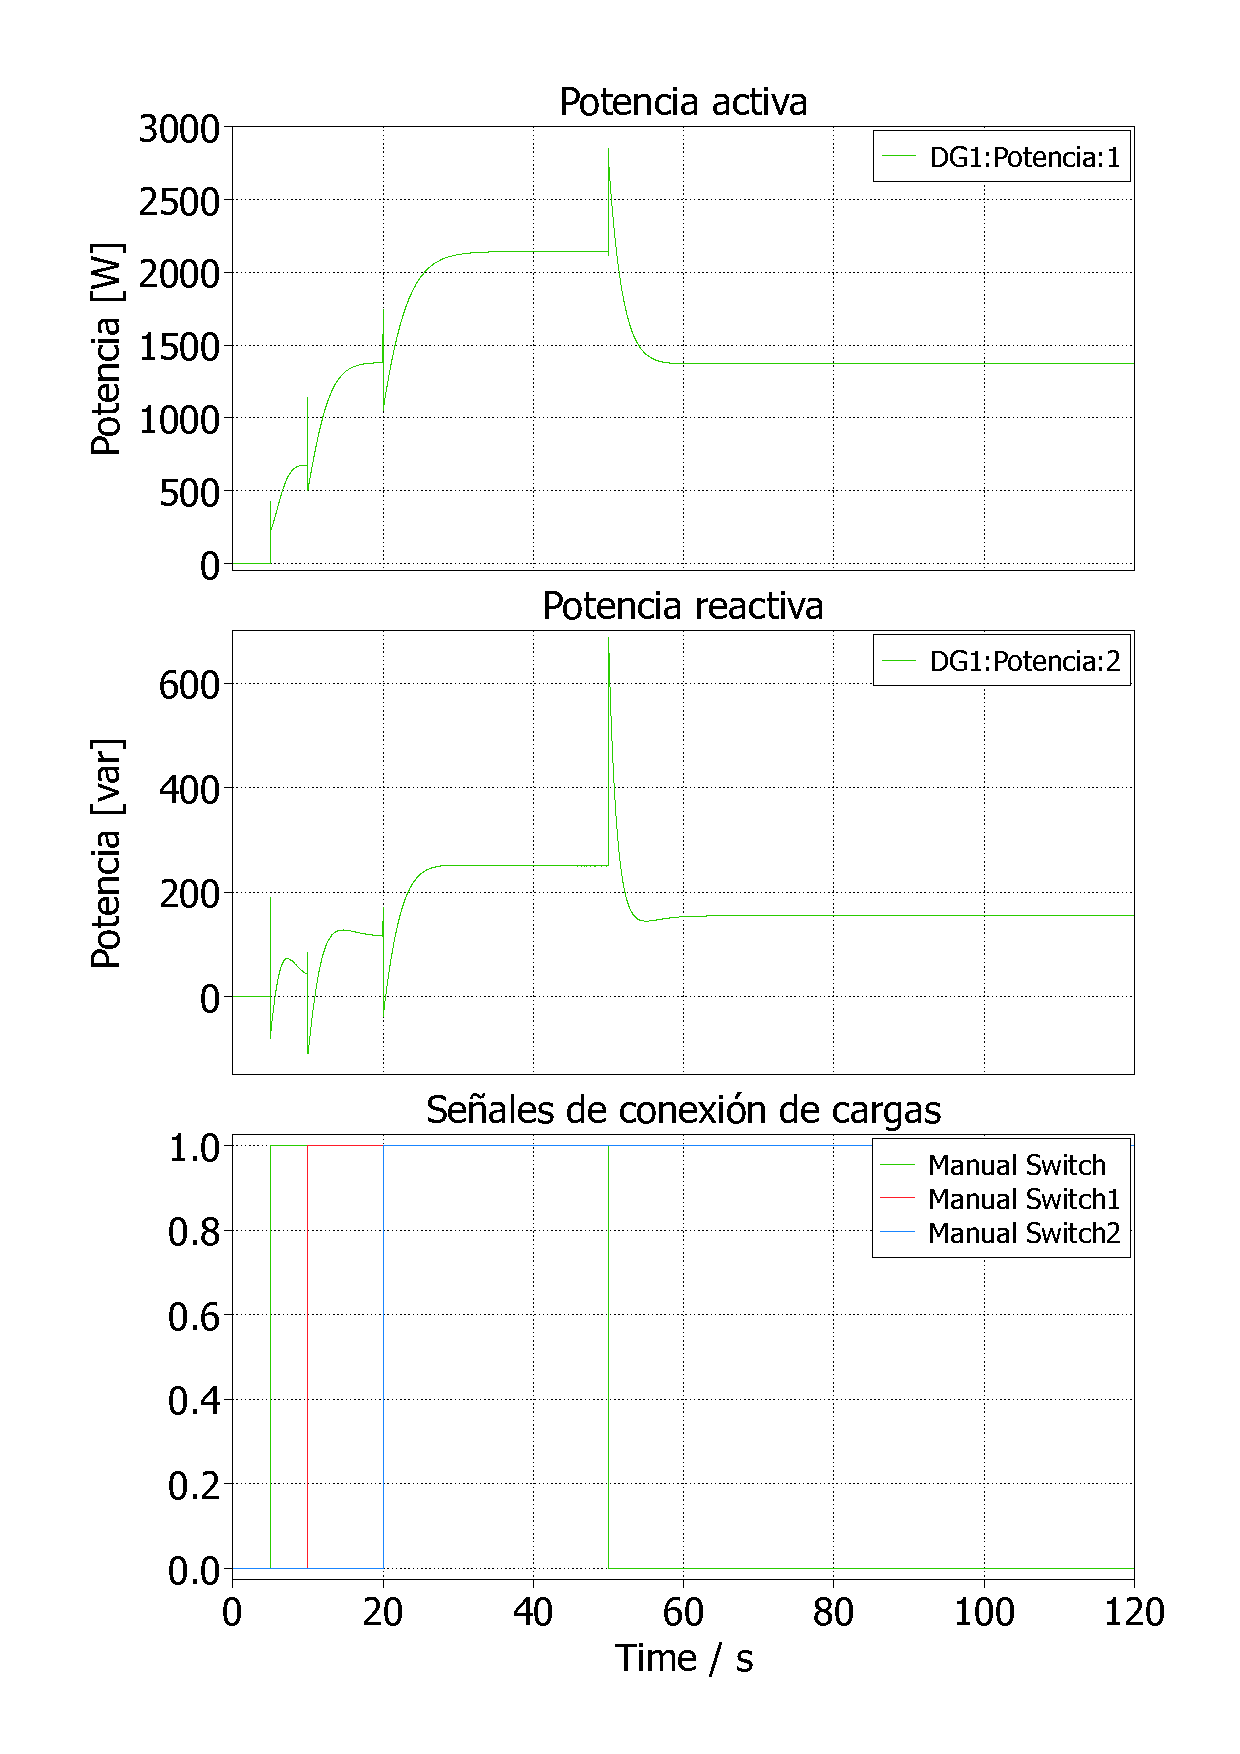
\includegraphics[width=0.5\linewidth]{Tarea 1/report/imagenes/p3a/droop_1.pdf}
   \caption{Potencia calculada con $Mp = -0.0005$ y $Mq_-0.0018$.}
   \label{droop_1}
\end{figure}

\begin{figure}
   \centering
   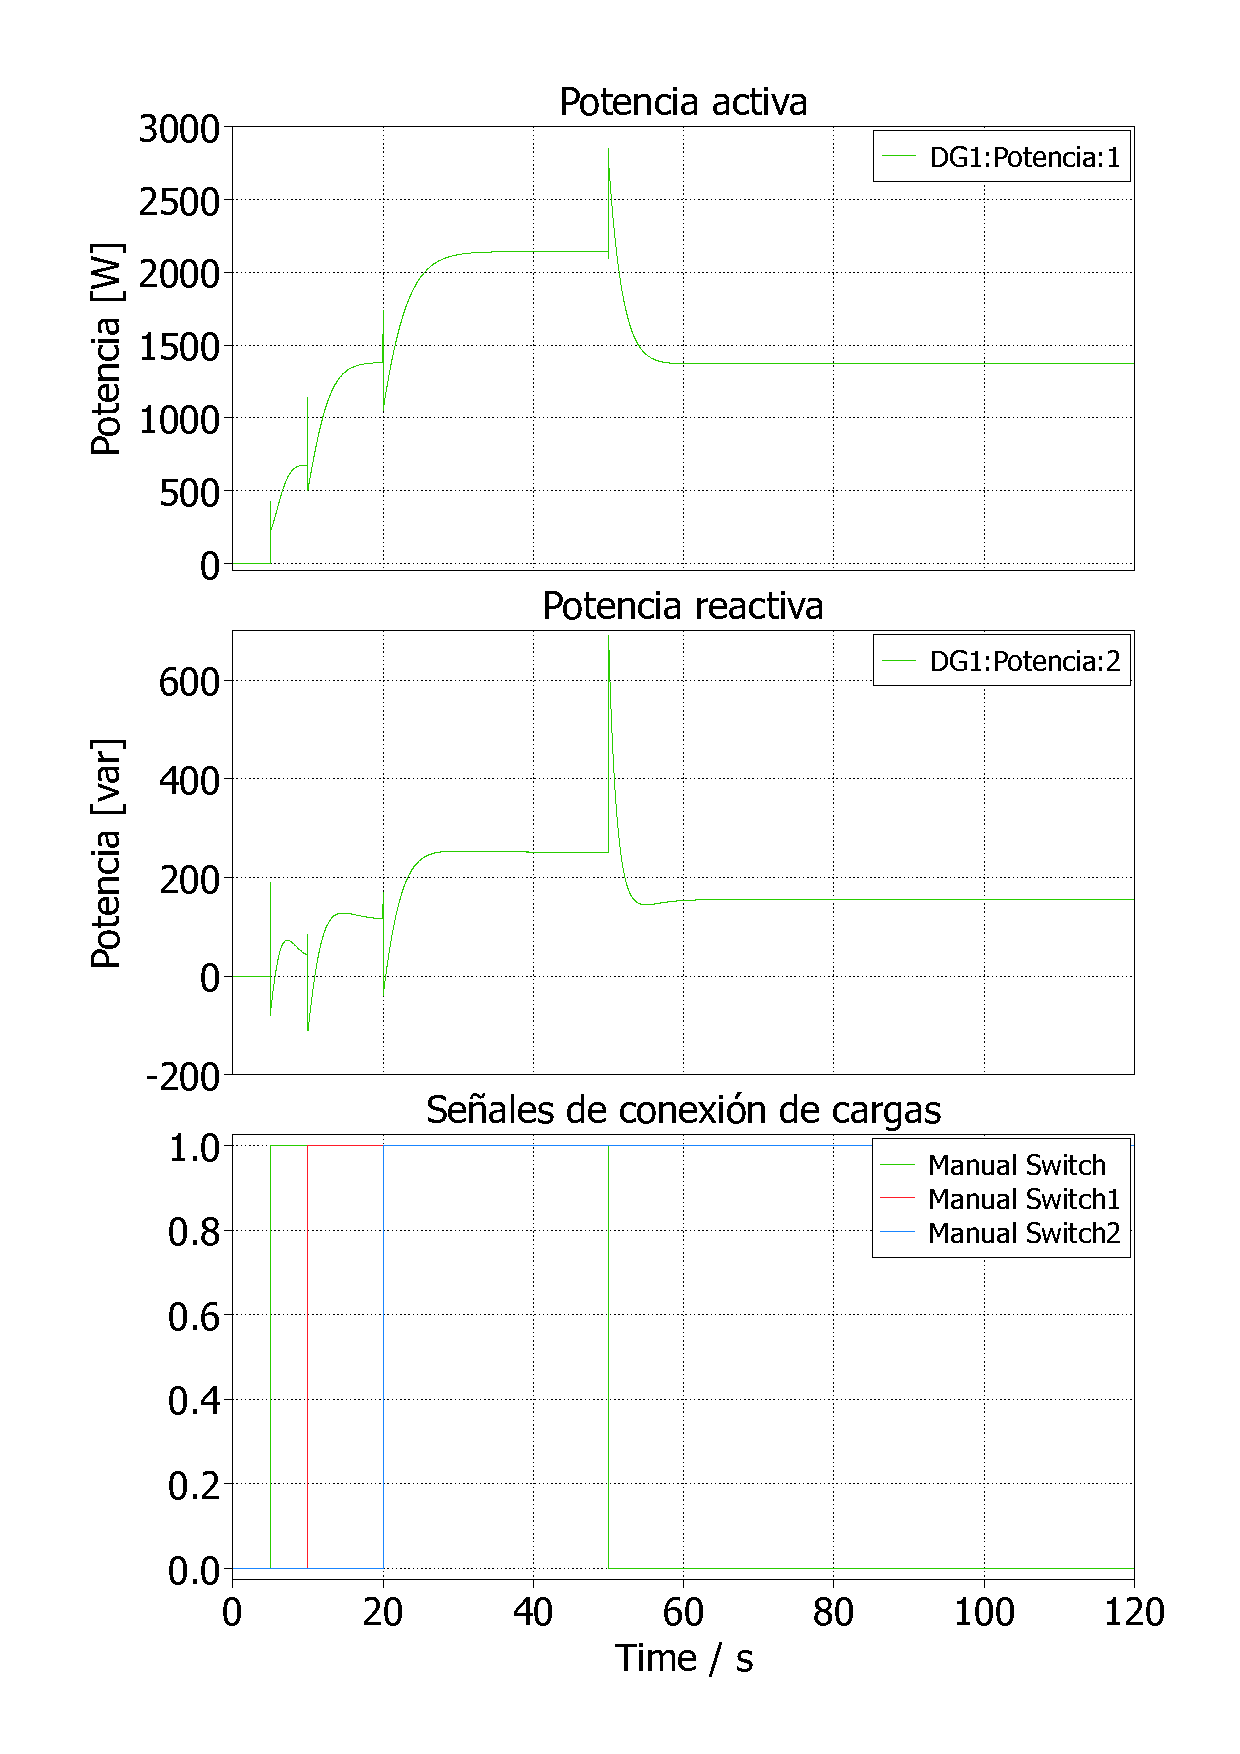
\includegraphics[width=0.5\linewidth]{Tarea 1/report/imagenes/p3a/droop_2.pdf}
   \caption{Potencia calculada con $Mp = -0.0003$ y $Mq_-0.0018$.}
   \label{droop_2}
\end{figure}

\begin{figure}
   \centering
   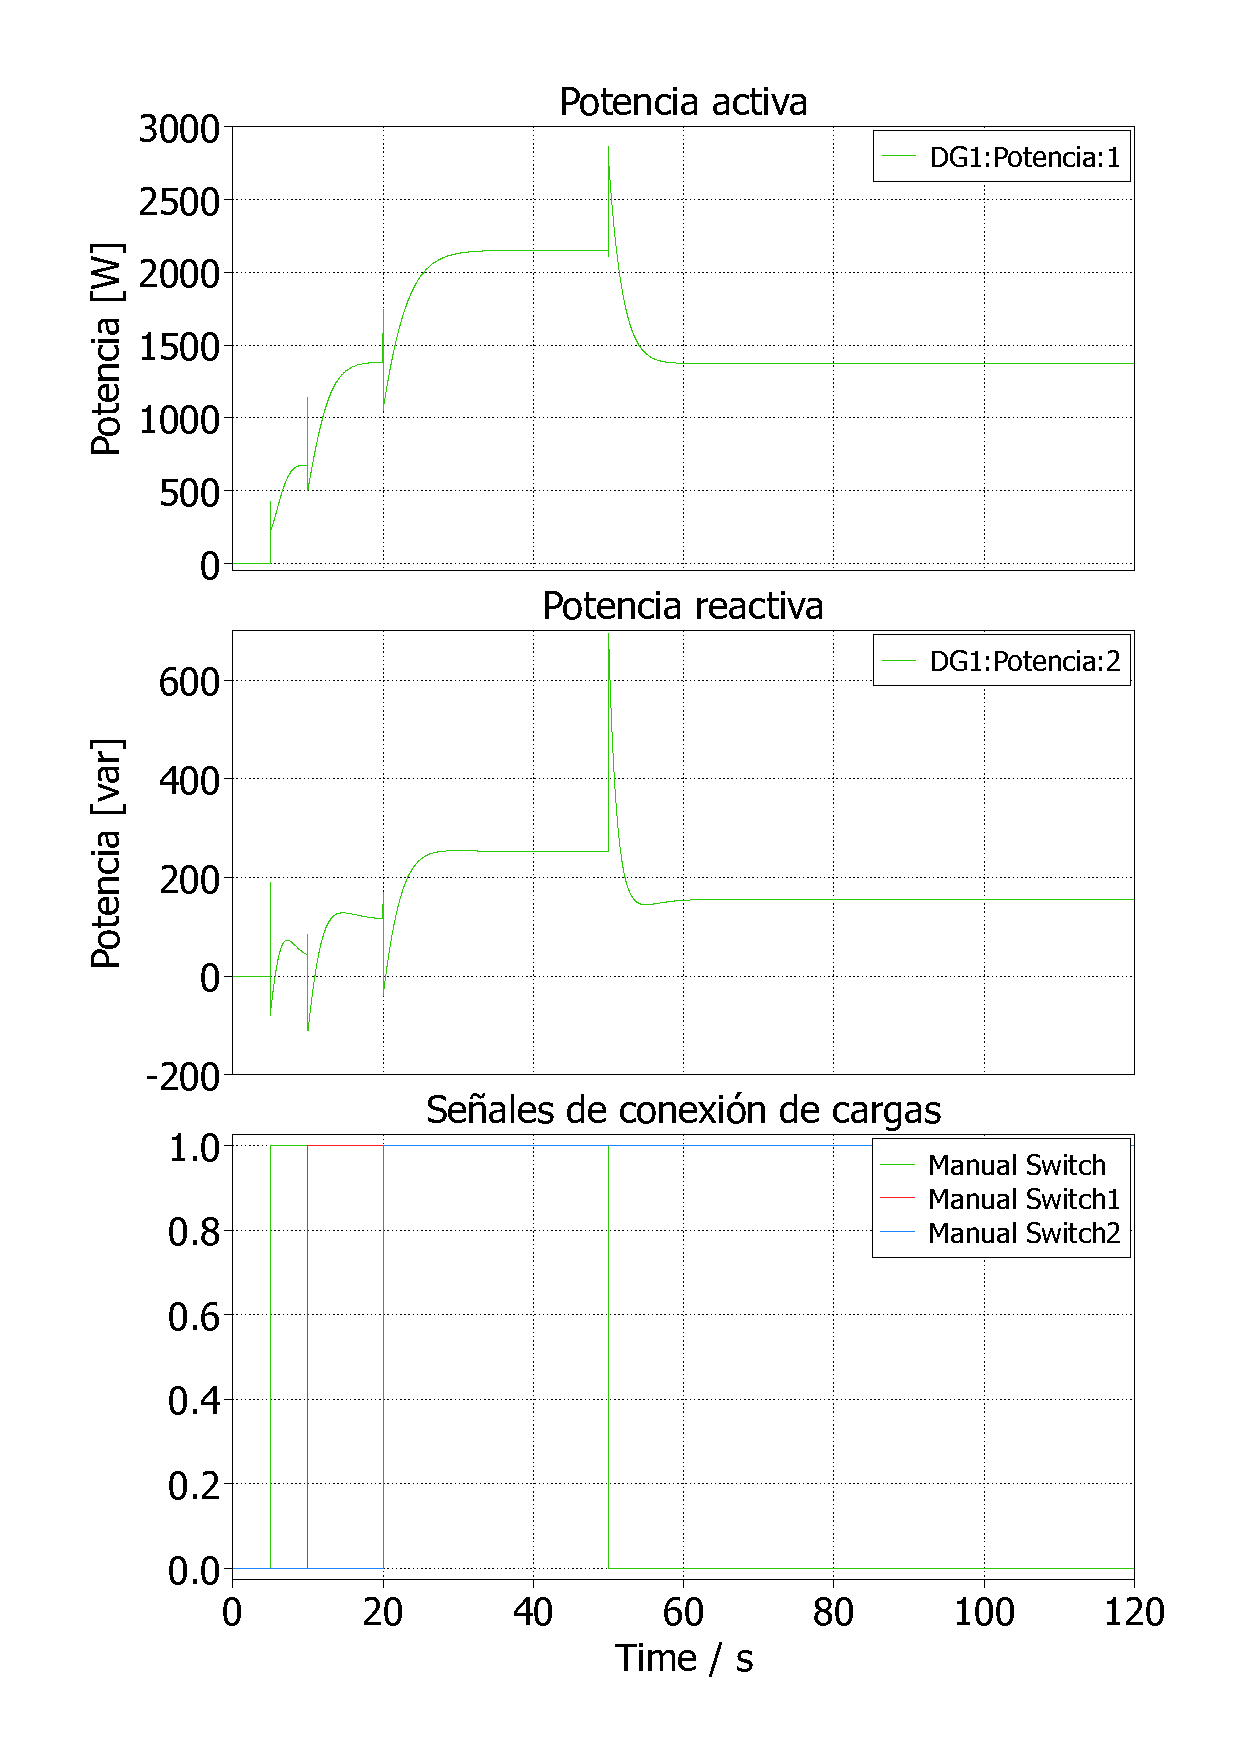
\includegraphics[width=0.5\linewidth]{Tarea 1/report/imagenes/p3a/droop_3.pdf}
   \caption{Potencia calculada con $Mp = -0.000036$ y $Mq_-0.0018$.}
   \label{droop_3}
\end{figure}

Se puede observar a partir de estas que la variación de las pendientes \textit{droop}, en una sola unidad

\subsection{Parte b.-}

Siguiendo las instrucciones, se cambiaron las pendientes droop de potencia activa y reactiva de modo que cada unidad generadora tiene valores de pendientes distintas. De este modo, se obtuvieron los siguientes resultados:



De acuerdo a estas simulaciones, la potencia...

\subsection{Parte c.-}

Investigando lo pedido, en el artículo 5-62 de la Norma Técnica de Seguridad y Calidad de Servicio (NTSyCS) estrenada en Septiembre del 2020, se estipula que:\\

La evaluación del desempeño del Control de Frecuencia del SI se efectuará a través del cálculo del factor FECF para cada hora k, el cual se define a través de la siguiente expresión:

\begin{equation}
    FECF(k) = 1 - \abs{\frac{\Delta f^*_{máx}(k)}{\Delta f_{máx}}}
\end{equation}

Donde:

\begin{itemize}
    \item $\Delta f^*_{máx}(k)$: Desviación máxima instantánea del valor filtrado de medición de la frecuencia.
    \item $\Delta f_{máx}$: Desviación máxima de frecuencia en estado permanente que agota la totalidad de la reserva asociada al Control Primario de Frecuencia y el Control Rápido de Frecuencia.
\end{itemize}

De acuerdo a esto, la pendiente máxima recomendada será la que entregue un FECF lo más cercana a 1 dado que este será el que entregará el mejor desempeño del Control de Frecuencia. Para lograr esto, lo que se requiere es que se tenga un $\Delta f^*_{máx}(k)$ lo más pequeño posible y un $\Delta f_{máx}$ lo más grande posible. Sin embargo, no fue posible encontrar valores que hicieran esto posible dado que no se dan datos de reservas ni del Control Rápido de Frecuencia.\\

Por otro lado, la pendiente droop es crucial para el control de potencia en sistemas eléctricos modernos, especialmente en redes descentralizadas como microrredes y sistemas con fuentes de energía distribuidas. Proporciona una solución efectiva, autónoma y estable para compartir la carga y regular las condiciones de operación sin la necesidad de un control centralizado o comunicación directa entre las unidades. Además, es esencial para manejar la variabilidad en sistemas que integran energías renovables, asegurando la estabilidad y eficiencia operativa.\\

\section{Pregunta 3}

\subsection{Parte a.-}

Se diseñó un PLL de acuerdo a las especificaciones recomendadas en las clases del curso, este fue colocado en la red con el fin de medir su frecuencia, el diseño se encuentra a continuación:

\begin{figure}
   \centering
   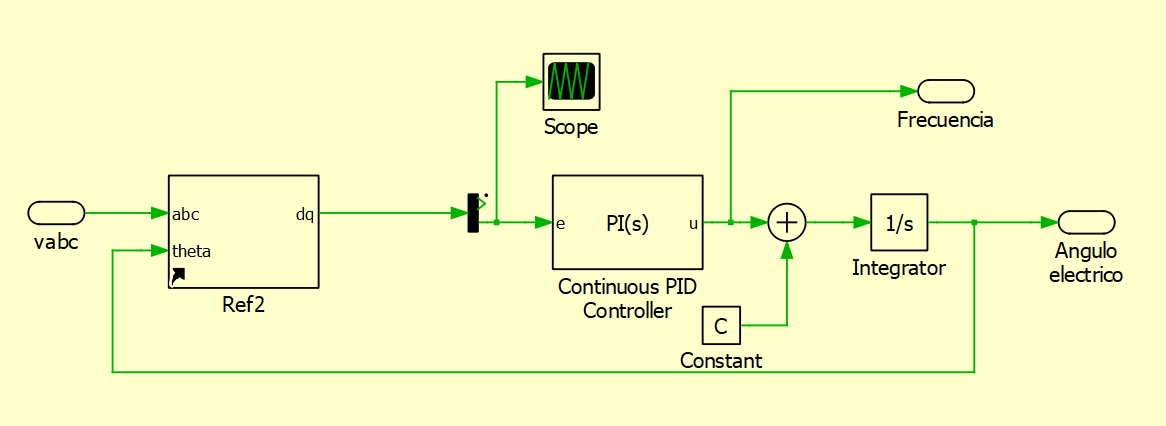
\includegraphics[width=0.5\linewidth]{Tarea 1/report/imagenes/p3a/pllred.png}
   \caption{Diseño PLL.}
   \label{diseñopll}
\end{figure}

El controlador PI utilizó las fórmulas:

\begin{equation}
    k_p = 2\zeta w_{n}
\end{equation}

\begin{equation}
    k_i = w_{n}^2
\end{equation}

Donde los valores utilizados para el coeficiente de amortiguamiento $\zeta$ y la frecuencia natural $w_{n}$ fueron 0.82 y 25 Hz respectivamente.\\

En base a esto, se realizó una simulación donde las 3 unidades de generación parten desconectadas y luego se conectan las 3 al mismo tiempo, los resultados fueron los siguientes:



Las mediciones otorgadas por el PLL indican que la frecuencia de la red toma un valor entre los rangos de X y Z, esto implica que...

\subsection{Parte b.-}

De acuerdo a lo pedido, se diseñó un controlador secundario que restaura la frecuencia de la red, su diseño se encuentra a continuación:

\begin{figure}
   \centering
   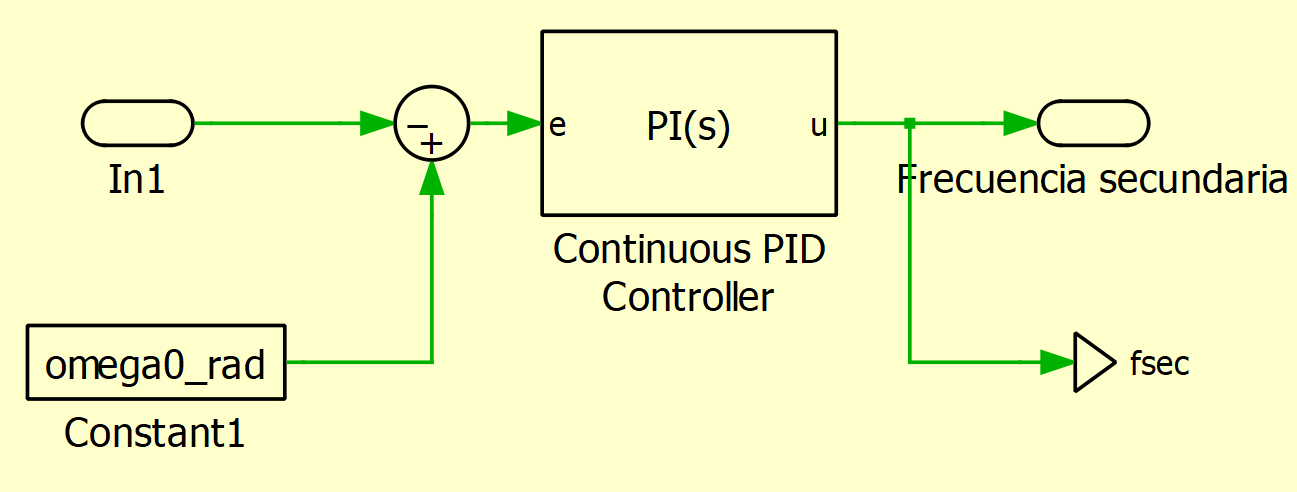
\includegraphics[width=0.5\linewidth]{Tarea 1/report/imagenes/p3b/secundario frecuencia.png}
   \caption{Diseño de controlador secundario de frecuencia.}
   \label{diseñosecfrecuencia}
\end{figure}

El controlador PI diseñado utilizó las mismas fórmulas de la parte a.-. Sin embargo, de acuerdo a las recomendaciones dadas en cátedra, el control secundario mantiene el rango de operación del coeficiente de amortiguamiento que se utilizó en los demás PI pero opera con anchos de banda entre los 0.2 Hz y 1 Hz, por lo que se decidió ocupar un coeficiente de amortiguamiento de 0.82 y una frecuencia natural de 0.6 Hz. Dado que el control secundario opera a una frecuencia 10 veces menor que el control droop, se considera que este está desacoplado del control primario.

\subsection{Parte c.-}

De acuerdo a lo pedido, se diseñó un controlador secundario que restaura el voltaje para el promedio de tensión de la red, su diseño se encuentra a continuación:

\begin{figure}
   \centering
   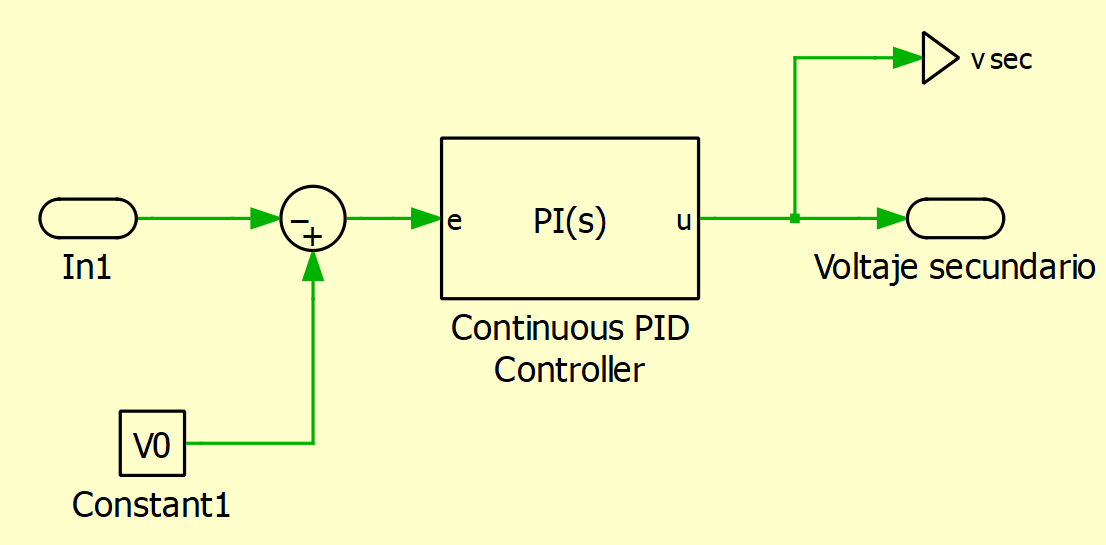
\includegraphics[width=0.5\linewidth]{Tarea 1/report/imagenes/p3c/secundario voltaje.png}
   \caption{Diseño de controlador secundario de voltaje.}
   \label{diseñosecvoltaje}
\end{figure}

El controlador PI diseñado utilizó las mismas fórmulas de la parte a.-. Sin embargo, de acuerdo a las recomendaciones dadas en cátedra, el control secundario mantiene el rango de operación del coeficiente de amortiguamiento que se utilizó en los demás PI pero opera con anchos de banda entre los 0.2 Hz y 1 Hz, por lo que los valores del controlador son los mismos que los utilizados para el PI del control secundario de frecuencia.\\

Al realizar simulaciones con el controlador secundario de voltaje, se obtuvo que...

\subsection{Parte d.-}



\section{Extras}

\subsection{Parte a.-}



\subsection{Parte b.-}



